\documentclass{sig-alternate}

% Include needed packages
\usepackage{graphicx}             	    % Needed for including graphics in EPS
\usepackage{cite}                        % Needed for doing citations
\usepackage[noend]{algorithm,algorithmic}% Needed for algorithms	
\usepackage{multirow,multicol,longtable} % Multiple rows/cols in tables
\usepackage{subfigure}                   % Needed for subfigures

% Notation
\newcommand{\cR}{{\cal R}}
\newcommand{\cE}{{\cal E}}
\newcommand{\cA}{{\cal A}}
\newcommand{\cD}{{\cal D}}
\newcommand{\cM}{{\cal M}}
\renewcommand{\bf}{{\mathbf f}}
\newcommand{\bs}{{\mathbf s}}
\newcommand{\bx}{{\mathbf x}}
\newcommand{\bone}[2]{\mathbf{1}_{#1}(#2)}
\newcommand{\bones}{\mathbf{1}}
\newcommand{\bzero}{\mathbf{0}}
\newcommand{\bmu}{{\boldsymbol \mu}}
\newcommand{\bsigma}{{\boldsymbol \Sigma}}
\newcommand{\bpi}{{\boldsymbol \pi}}
\newcommand{\bphi}{{\boldsymbol \phi}}
\newcommand{\bbeta}{{\boldsymbol \beta}}
\newcommand{\figref}[1]{\mbox{Figure \ref{#1}}}
\newcommand{\PBILc}{\texttt{PBIL$_c$}}
\newcommand{\cGA}{\texttt{cGA}}
\newcommand{\EDA}{\texttt{EDA}}
\newcommand{\TILDA}{\texttt{TILDA}}
\newcommand{\TILDAC}{\texttt{@TILDA}}
\newcommand{\onemax}{\texttt{OneMax}}
\newcommand{\rroad}{\texttt{RoyalRoad}}
\newcommand{\noisy}{\texttt{Noisy~}}
\newcommand{\tgauss}[2]{{\cal N}^{\mathsf{\,T}}(#1, #2)}
\newcommand{\transpose}{\mathsf{T}}
\newcommand{\gauss}[2]{{\cal N}(#1, #2)}
\newcommand{\Rdom}{\mbox{$\mathbb{R}$}}
\floatname{algorithm}{Algorithm}
\renewcommand{\algorithmicrequire}{\textbf{Requires:}}
\renewcommand{\algorithmicensure}{\textbf{Outputs:}}
\renewcommand{\algorithmicfor}{\textbf{repeat}}
\renewcommand{\algorithmicwhile}{\textbf{repeat until}}
\renewcommand{\algorithmicdo}{\textbf{}}
\renewcommand{\algorithmiccomment}[1]{#1}
\algsetup{indent=1em}

\begin{document}
 \conferenceinfo{GECCO'12,} {July 7-11, 2012, Philadelphia, Pennsylvania, USA.}
 \CopyrightYear{2012}
 \crdata{978-1-4503-1177-9/12/07}
 \clubpenalty=10000
 \widowpenalty =10000

\title{A Memory Efficient and Continuous-valued Compact EDA for Large Scale Problems}
%\subtitle{[Extended Abstract]
%

\numberofauthors{2} 
\author{
\alignauthor
Sergio Rojas-Galeano\\
       \affaddr{Engineering School}\\
       \affaddr{District University of Bogota}\\
       \affaddr{Bogota, Colombia}\\
       \email{srojas@udistrital.edu.co}
\alignauthor
Nestor Rodriguez\\
       \affaddr{Engineering School}\\
       \affaddr{District University of Bogota}\\
       \affaddr{Bogota, Colombia}\\
       \email{nearodriguezg@correo.udistrital.edu.co}
}
\date{\today}
\maketitle

\begin{abstract}
This paper considers large-scale \onemax~and \rroad~optimization problems with up to $10^7$ binary variables within a \emph{compact} Estimation of Distribution Algorithms (\EDA) framework. Building upon the compact Genetic Algorithm (\cGA), the continuous domain Population-Based Incremental Learning algorithm (\PBILc) and the arithmetic-coding \EDA, we define a novel method that is able to compactly solve regular and noisy versions of these problems with minimal memory requirements, regardless of problem or population size. This feature allows the algorithm to be run in a conventional desktop machine. Issues regarding probability model sampling, arbitrary precision of the arithmetic-coding decompressing scheme, incremental fitness function evaluation and updating rules for compact learning, are presented and discussed.
\end{abstract}

\category{I.2.8}{Computing Methodologies}{Artificial Intelligence}[Problem Solving, Control Methods and Search]

\terms{Algorithms}

\keywords{EDA, compact GA, large scale optimization, \mbox{arithmetic coding}}

\section{Introduction}
Estimation of Distribution Algorithms (\EDA) \cite{Larranaga01, Pelikan06} approximately optimizes a cost function by building a probabilistic model of a pool of promising sub-optimal solutions over a given search space. For very-high dimensional search spaces, storing and updating a large population of candidates may imply a computational burden in both time and memory. The \emph{compact} approach circumvents storage limitations by incrementally updating the probability model using just two candidates at any step of the algorithm, instead of the entire population. This feature makes the compact \EDA~framework practical for large-scale optimization, a soon-to-be commonplace setting in scientific domains such as bioinformatics, particle physics, chemical crystallography, or social network analysis, to name a few.

This study reports on a new efficient, continuous-valued, compact \EDA~aimed at optimization of large-scale problems of up to $10^7$ binary decision variables, nevertheless requiring low-cost computational resources. The method is tailored to optimization of decomposable cost functions in terms of the contribution of individual variables, that is, to problems where incremental fitness evaluation is feasible. Although at present no second- or higher-order dependencies within the variables are considered in our method, its value as an early-stage data analysis tool in high dimensional spaces might be relevant, for example to carry out feature selection for subsequent dependencies estimation on smaller variable subsets, as other models with independence assumptions have shown\cite{Rojas08}. Even so, we anticipate modeling multivariate dependencies will widen the applicability of our method. In this respect, incorporating memory and time efficiencies such as fitness evaluation relaxation\cite{Sastry02} would be an interesting avenue of future work.   

Our findings are organized as follows: a short review of methods related to our research is presented in section \ref{sec:review}; a description of the techniques involved in the design of the algorithm is given in section \ref{sec:tools}; the algorithm itself is discussed in section \ref{sec:algorithm}; empirical arguments are provided in section \ref{sec:experiments} and closing remarks are highlighted in section \ref{sec:conclusion}.

\textbf{Notation}. Lower-case boldface is used to denote vector arrays (e.g. ${\boldsymbol \mu} \in \Rdom^2, \bs \in \Rdom^\ell$) whereas plain font denotes scalar values (e.g. $\gamma, p, q \in \Rdom$). Capital letters refer to sets of elements. We use $n$ to denote the size of a given population, and $\ell$ represents the size of the search problem, that is, its dimensionality. 

\section{Literature review}
\label{sec:review}
The compact Genetic Algorithm (\cGA)\cite{Harik99} was proposed as a memory-efficient variant of the canonical genetic algorithm\cite{Goldberg89}. The idea behind the \cGA~is to consider the population of candidates as a sample from which a probability model of Bernoulli trials can be estimated. The algorithm performs successive binary tournaments of two sampled candidates from the current distribution and also updates the model parameters with a frequentist rule based on only those two candidates; thus it avoids the need to keep the entire population in memory. As a result, the \cGA~reduces the storing capacity needed to evolve the population from $O(n\ell)$ to $O(\ell(\log_2 n+2))$. This property enabled the algorithm to solve problems with dimensionality up to one billion binary variables, as subsequently reported in \cite{Sastry07}. In such problems ($\ell=10^9, \log_2 \ell \approx 30$), the memory size required for running the algorithm would roughly reach $(10^9 \times 32)\mathrm{bits} \approx 3,72\mathrm{Gb}$, yet a stringent amount for a conventional machine; in fact, some efficacies including distributed computing, vectorized and integer operations, and tailored random number generation were necessary to solve large scale problems with a \cGA~running in a 256-processor cluster machine\cite{Sastry07}.  

\cGA~works in discrete domains where variables take binary values. Other non-compact \EDA s have been proposed to address optimization in both discrete\cite{Baluja95, Muhlenbein97} and continuous domains\cite{Sebag98, Larranaga02}. Particularly, continuous-domain Population-Based Incremental Learning (\PBILc) \cite{Sebag98} is an algorithm that assumes variables are independently normally distributed. The mean and variance parameters are updated using the maximum likelihood marginal estimates from a sample population. Since the population is used at every iteration of the algorithm, \PBILc~is more demanding in terms of memory when compared to \cGA, and would be difficult to apply to large scale problems in conventional machines.

It is also worth mentioning a recent study\cite{Suwannik08} where an encoding technique known as arithmetic-coding\cite{Said04}, was used within a continuous domain population-based \EDA~to solve large scale problems of up to one billion variables. The encoding technique allows compressing a binary string of arbitrary length using a couple of double precision numbers. Although the fitness evaluation still requires $\ell/8$ bytes of memory per active candidate, the compression scheme enabled the algorithm to solve the problem with a population size of $3200$ candidates in a regular PC-computer in about 36 hours. Regrettably, the study did not provide details on the mechanics of the algorithm, motivation of the updating rules of the distribution parameters, or issues related to the precision of arithmetic-coding.

In this paper we build upon the above algorithms and propose a novel method to solve canonical and noisy versions of large-scale \onemax~and \rroad~ problems by using a compact and continuously-valued representation, which is further enhanced with an arithmetic-coding scheme. For this kind of additively-separated tasks and with the assumption of independently-distributed binary variables, the new method demands minimal memory consumption ($O(1)$), regardless of the problem dimension or population size. The insights are reported in the following sections.

\section{Tools}
\label{sec:tools}

\subsection{TILDA}
\label{sec:tilda}
The basis of this study is an algorithm we devised as a mix of \cGA~and \PBILc. The underlying idea is to model the pool of solution candidates with a multivariate marginal joint Gaussian distribution whose parameters are estimated within a compact framework. The estimates of marginal parameters $(\mu_i, \sigma_i)_{i=1}^{\ell}$ for both the mean and standard deviation of each input variable, are periodically updated with information from the fittest candidates selected by means of 2-way tournaments, as explained next\footnote{A similar reasoning was followed in \cite[Appendix A]{Mininno08}.}. Let us assume we have a population $P$ of $2n$ candidates were $n$ simple 2-way tournaments are performed (two candidates from $P$ are randomly chosen without replacement, and the the winner substitutes the loser). Let $W$ and $L$ be the sets of tournament's winners and losers, respectively. The new population is then $\widetilde{P} = (P \setminus L) \cup W$. Then, the maximum likelihood mean estimate of the new population, that is $\bmu=(\mu_1,\ldots,\mu_\ell)$, can be computed in vectorized form as:
\begin{eqnarray*}
\boldsymbol \mu &=& \frac{1}{2n}\sum_{\bx_k \in \widetilde{P}}{\bx_k} = \frac{1}{2n} \left( \sum_{\bx_k \in P}{\bx_k} - \sum_{\bx_k \in L}{\bx_k} + \sum_{\bx_k \in W}{\bx_k}\right) \\ &=& \frac{1}{n} \sum_{\bx_k \in W}{\bx_k},
\end{eqnarray*}
since $P = W \cup L$. Now, assuming that variables are mutually independent, and defining the unordered set of winner indexes as ${\cal W}=\{k_t: t=1,\ldots,n;\; \bx_{k_t} \in W\}$, the estimate can be re-casted in terms of its components as: 
\begin{equation}
\mu_i=\frac{1}{n}\sum_{t=1}^n x_i^{k_t}, \nonumber
\end{equation}
where $x^{k_t}_i$ is the $i$-th component of the candidate $\bx_{k_t}$. We observe that if we initialise $\mu_i=0$, then the estimate can be updated incrementally with a fraction of each tournament's winner, as the formula in Equation (\ref{eq:mu}) indicates. 
\begin{equation}
\mu_i:=\mu_i+\tfrac{1}{n} x_i^{k_t}; \quad t=1,\ldots,n. \label{eq:mu}
\end{equation}

Now, the same rationale can be applied to the variance estimate $\bsigma=(\sigma_1^2, \ldots, \sigma_\ell^2)$: 
\begin{eqnarray}
\sigma_i^2 &=& \frac{1}{n} \sum_{t=1}^n (x^{k_t}_i-\mu_i)^2 = \frac{1}{n} \left( \sum_{t=1}^n (x^{k_t}_i)^2 - 2\mu_i \sum_{t=1}^n x^{k_t}_i + n \mu_i^2 \right) \nonumber \\
&=& \frac{1}{n} \sum_{t=1}^n (x^{k_t}_i)^2 - \mu_i^2. \label{eq:sigma0} \nonumber
\end{eqnarray}
Then again, an incremental update can be obtained by first setting a temporal variable $\tilde{\sigma}_i^2=0$, then accumulating deviations of each tournament's winner in this variable using Equation (\ref{eq:sigma1}), and finally subtracting the square of the previously computed mean estimate to obtain the variance estimate, as in Equation (\ref{eq:sigma2}). 
\begin{eqnarray}
\tilde{\sigma}_i^2 &:=& \tilde{\sigma}_i^2+\tfrac{1}{n} (x_i^{k_t})^2; \quad t=1,\ldots,n. \label{eq:sigma1} \\
\sigma_i^2 &=& \tilde{\sigma}_i^2-\mu_i^2 \label{eq:sigma2}
\end{eqnarray}
Equations (\ref{eq:mu}-\ref{eq:sigma2}) outline the compact updating rules of the new method, named the Tiny Incremental Learning Density Estimation Algorithm (\TILDA) -- see Algorithm \ref{alg:TILDA}.  
 
\begin{algorithm}
	\caption{\TILDA} 
	\begin{algorithmic}[1]
	\REQUIRE{$\ell>0$, fitness function $f(\cdot)$}
	\ENSURE{best candidate $\bbeta$}
		\STATE $\bmu=\bzero, \bsigma=\bones, \bbeta=\bzero, \gamma=0.5, \epsilon=0.01$
		\WHILE{\textbf{ending citeria not met}} \label{tilda:genloop}
			\STATE $\tilde{\bmu}=\tilde{\bsigma}=\bzero$
			\FOR{$n$ \textbf{times}} \label{tilda:poploop}
				\STATE $\{\bx^{\prime},\bx^{\prime\prime}\} \sim \gauss{\bmu}{\bsigma}$ \label{acGA:sampling} \label{tilda:sampling}
				\STATE $\hat{\bx} = \mathsf{argmax}(f(\bx^{\prime}), f(\bx^{\prime\prime}))$ \label{tilda:2way}
				\STATE $\bbeta = \mathsf{argmax}(f(\bbeta), f(\hat{\bx}))$ \label{tilda:beta}
				\STATE $\tilde{\bmu} = \tilde{\bmu} + \frac{1}{n}(\hat{x}_1,\hat{x}_2,\ldots,\hat{x}_{\ell})$ \label{tilda:muhat}
				\STATE \vspace{1mm}$\tilde{\bsigma} = \tilde{\bsigma} + \frac{1}{n}(\hat{x}_1^2,\hat{x}_2^2,\ldots,\hat{x}_{\ell}^2)$	 \label{tilda:sigmahat}
			\ENDFOR			
			\STATE $\bmu=\bmu-\gamma(\bmu-\frac{1}{2}(\bbeta+\tilde{\bmu}))$ \label{tilda:mu}
			\STATE $\bsigma=\bsigma-\gamma(\bsigma-(\tilde{\bsigma}-(\tilde{\mu}_0^2, \tilde{\mu}_1^2,\ldots, \tilde{\mu}_{\ell}^2))+\epsilon$	 \label{tilda:sigma}		
		\ENDWHILE
	\end{algorithmic}  
	\label{alg:TILDA}
\end{algorithm}
The aim of the algorithm is to approximately find a solution to the unconstrained optimisation problem:
$$\bbeta^\star=\underset{\bx \in \Rdom^\ell}{\mathsf{argmax}} \;f(\bx),$$
where $f(\cdot)$ is the fitness or cost function to be optimised. The algorithm models a population of promising solutions using a multivariate marginal joint Gaussian distribution with parameters $\bmu$ and $\bsigma$. The main loop (line \ref{tilda:genloop}) runs for a number of generations or until the parameters converge. The inner loop (line \ref{tilda:poploop}) simulates the breeding of one population by sampling two candidates at a time (line \ref{tilda:sampling}), carrying out 2-way tournaments to determine the winner $\hat{\bx}$ (line \ref{tilda:2way}), and also keeping temporary parameter estimates for the current population (lines \ref{tilda:muhat}-\ref{tilda:sigmahat}) using Equations (\ref{eq:mu}-\ref{eq:sigma1}). Notice that the algorithm stores the best solution found up to a certain generation in the variable $\bbeta$ (line \ref{tilda:beta}). The actual updates of the overall estimates are performed at the end of the main loop (lines \ref{tilda:mu}-\ref{tilda:sigma}). The overall mean estimate is computed with a memory-preserving rule with decay factor $\gamma$, incorporating an elitist mechanism that shifts the estimate towards the average of the population mean and the best candidate. Similarly, the overall variance estimate uses the population mean, as stated in Equation (\ref{eq:sigma2}), plus a small constant intended to prevent premature convergence\footnote{It is interesting to remark that more sophisticated mechanisms to prevent premature convergence such as adaptive variance scaling from \EDA~and Evolutionary Strategies literature (e.g.\cite{Kramer11, Cai07, Back93}), are worthy of further study in future extensions.}. When the ending criteria is met, the approximate optimal solution found by the algorithm can be retrieved from $\bbeta$.

\subsection{Arithmetic coding of binary strings}
Given the alphabet $S=\{0,1\}$ and a probability distribution $\Phi=\{P(0)\!=\!p,P(1)\!=\!1-p\}$, the idea of arithmetic coding is to represent an arbitrary binary string of length $\ell$ using distribution $\Phi$ and a single real number $q \in [0,1]$ known as a \emph{code value} (see details in \cite{Said04}). Decoding is achieved by performing a Bernoulli trial for each bit in the sequence, that is, flipping an unfair coin with bias $p$, where $q$ represents the chance of a face-up outcome. For this purpose, the decoder builds nested intervals and biases $\{[a_i,b_i],p_i\}_{i=1}^{\ell}$ that re-define the support and probability distributions throughout consecutive bits along the sequence. Thus, a decoded string $\bs_p^q$ corresponds to $\bs_p^q = (s_i^q)_{i=1}^\ell = (s_1^q, \ldots, s_\ell^q)$, where the outcome for each bit $i$ is determined by the indicator function: 
%$$\bone{i}{q}= \left\{\begin{matrix} 1&& q \ge p_i \\ 0&& q < p_i \end{matrix} \right. ,$$
\begin{equation}
s_i^q= \left\{\begin{matrix} 0&& q \le p_i \\ 1&& q > p_i \end{matrix} \right. \,,\; i \ge 1, \label{eq:spi}
\end{equation}
and the bias $p_i$ is updated iteratively according to the outcome of the preceding bit and the bounds $a_i, b_i$ of the nested support intervals, following the recursions: 
\begin{equation}
\begin{array}{lll}
\left[a_1, b_1 \right] &=& [0, 1] \,, \\
\left[a_i, b_i \right] &=& \Bigg \{\begin{matrix} [a_{i-1}, p_{i-1}] && q \le p_{i-1} \\ [p_{i-1}, b_{i-1}] && q > p_{i-1} \end{matrix} \,,\; i>1, \\
p_i &=& a_{i}+(b_{i}-a_{i})p \,,\; i \ge 1.  
\end{array} 
\label{eq:aibipi}
\end{equation} 
Equation (\ref{eq:aibipi}) implies that the support interval for a subsequent trial is replaced by the subinterval chosen from the comparison of the code value and the bias of the current trial. As a result, the length of nested intervals shrinks away as the decoding progresses, with the values of these variables growing in precision digits. In theory, one may obtain an arbitrary number of bits with this decoding scheme. In practice, however, the number of bits is limited by machine-dependent floating point arithmetic, in other words, due to round-off errors the supporting interval (and the bias $p_i$ too) eventually collapses and yields the code value $q$, resulting in a constant zero-output from that trial onwards. 

In an attempt to circumvent this shrinking-interval limitation, we contemplated an alternative decoding scheme, as explained next. Firstly, observe that during the shrinking procedure the nested probability distributions obtained with the successive updates of $[a_i, b_i]$ and $p_i$, preserve the proportions of the original distribution defined by $p$ in $\Phi$. In fact, these are just shrunk replica distributions repeatedly shifted to different locations along the unit interval. Within these distributions, the \emph{global} (fixed) code value $q$ defines a \emph{local} chance of outcome that is relative to the location of the supporting interval and bias of the respective trial. Bearing in mind this observation, we sought to switch roles and keep distribution $\Phi$ \emph{global}, that is, fixed to the unit interval, whereas the otherwise constant code value is repeatedly shifted to mirror the \emph{local} chance of outcome at each trial of the shrinking procedure. In this way, for all $i$ we fixed $[a_i=0, b_i=1]$ and $p_i=p$ and rescaled the value of the now variable $q_i$ using the following recursive rules:
\begin{equation}
\begin{array}{lll} q_1 &=& q \,,\\ &&\\
q_i &=& \left\{ \begin{matrix} \dfrac{q_{i-1}}{p} && q_{i-1} \le p \\ 
\dfrac{(q_{i-1}-p)}{(1-p)} && q_{i-1} > p \end{matrix} \,,\; i>1 \right.
\end{array} \label{eq:qi}
\end{equation} 

In this new scheme, the values of $q_i$ shift around the unit interval resembling the cursor of an old-fashion sliding rule, thus the name \emph{sliding-pin} arithmetic decoding. Since the length and bias of the supporting interval are in a normal scale, the relocated values of $q_i$ are not machine-precision dependent. Additionally, it is worth noting that the sliding-pin procedure only maintains one parameter ($q_i$) as opposed to three parameters ($a_i,b_i,p_i$) for the shrinking decoding. The decoded string $\bs_p^q$ would be now obtained as:
\begin{equation}
\bs_p^q = (s_i^p)_{i=1}^\ell = (s_1^p, \ldots, s_\ell^p), \label{eq:spq}
\end{equation}
where the indicator function becomes: 
\begin{equation}
s_i^p= \left\{\begin{matrix} 0&& q_i \le p \\ 1&& q_i > p \end{matrix} \right. \,,\; i \ge 1. \label{eq:sqi}
\end{equation}
The two decompression schemes are illustrated in Figure \ref{fig:ac}.

\begin{figure}[H]
	\centering
	\subfigure[]{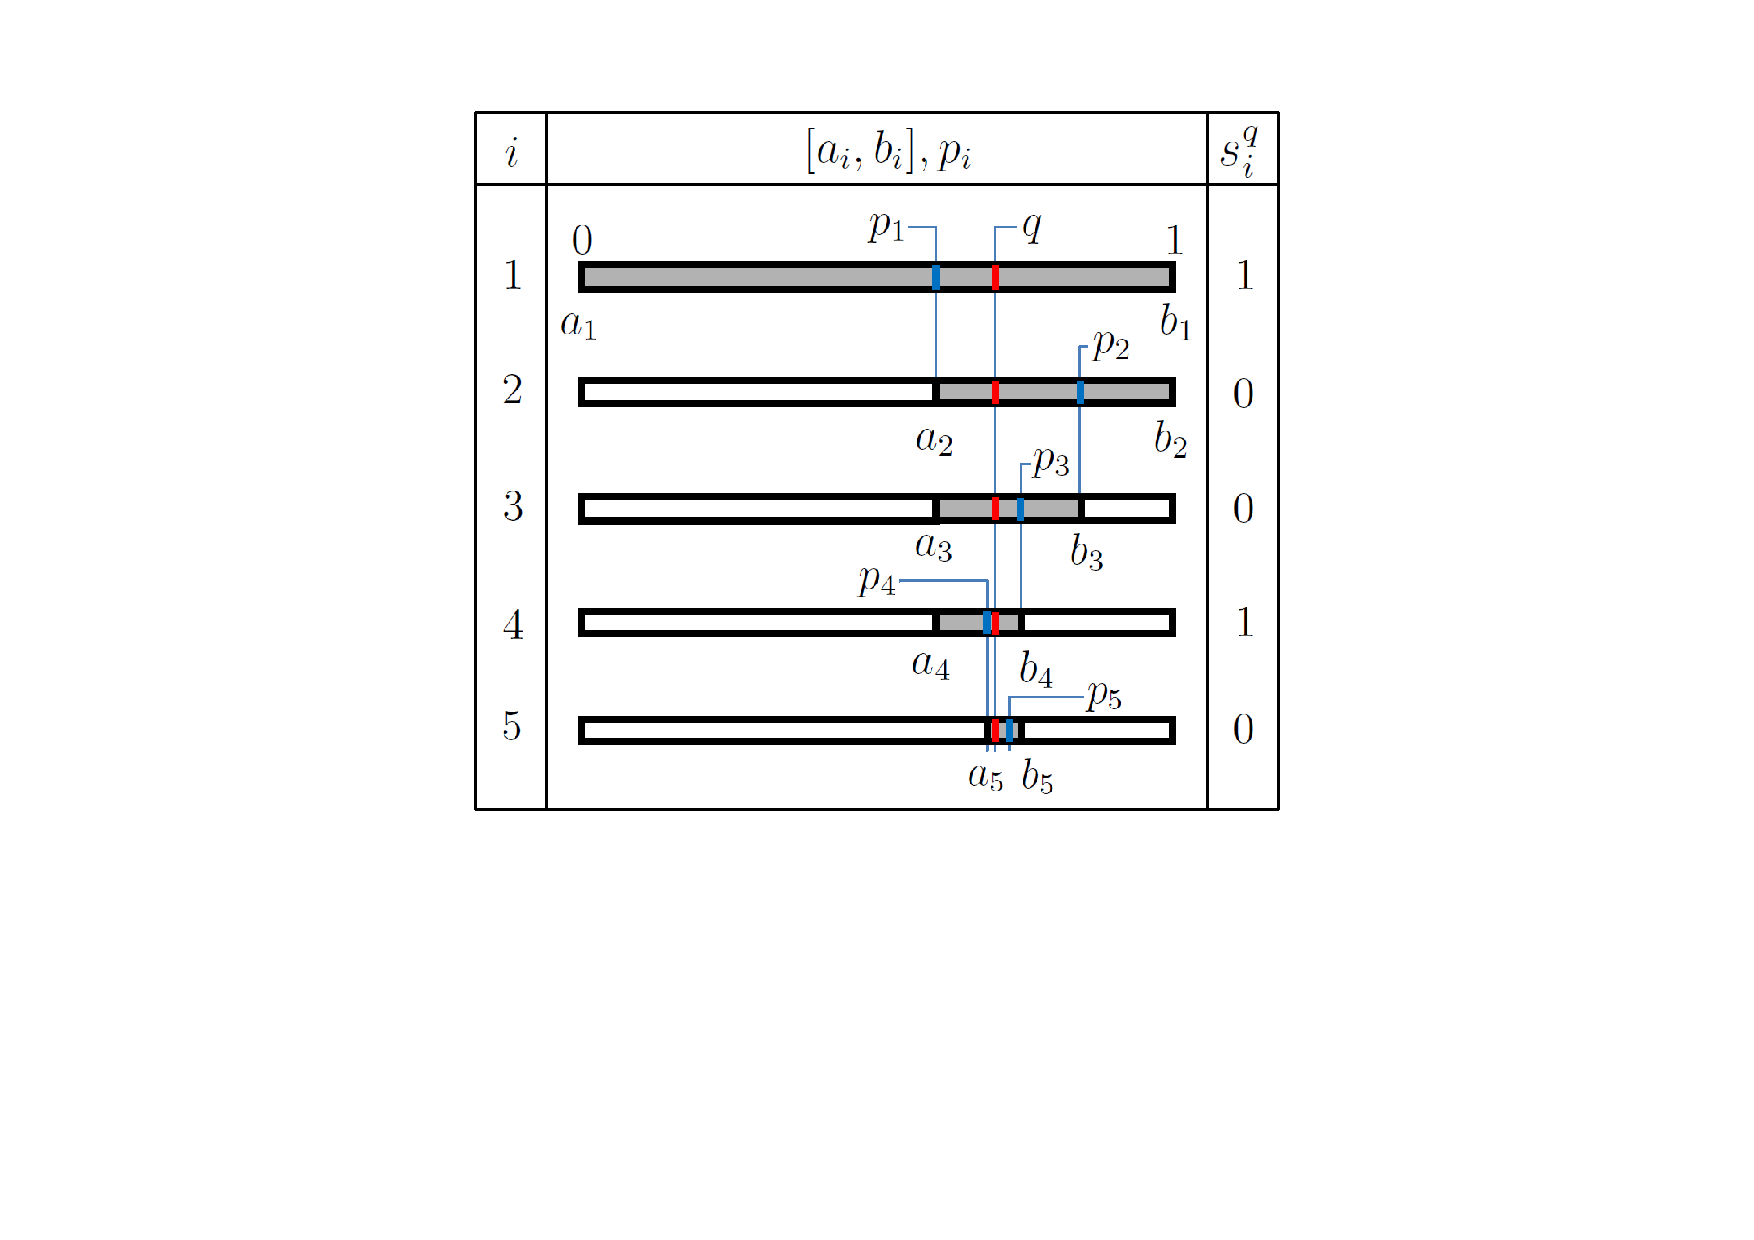
\includegraphics[scale=.5]{shrinking-interval-bw}\label{fig:shrinking}}
	\subfigure[]{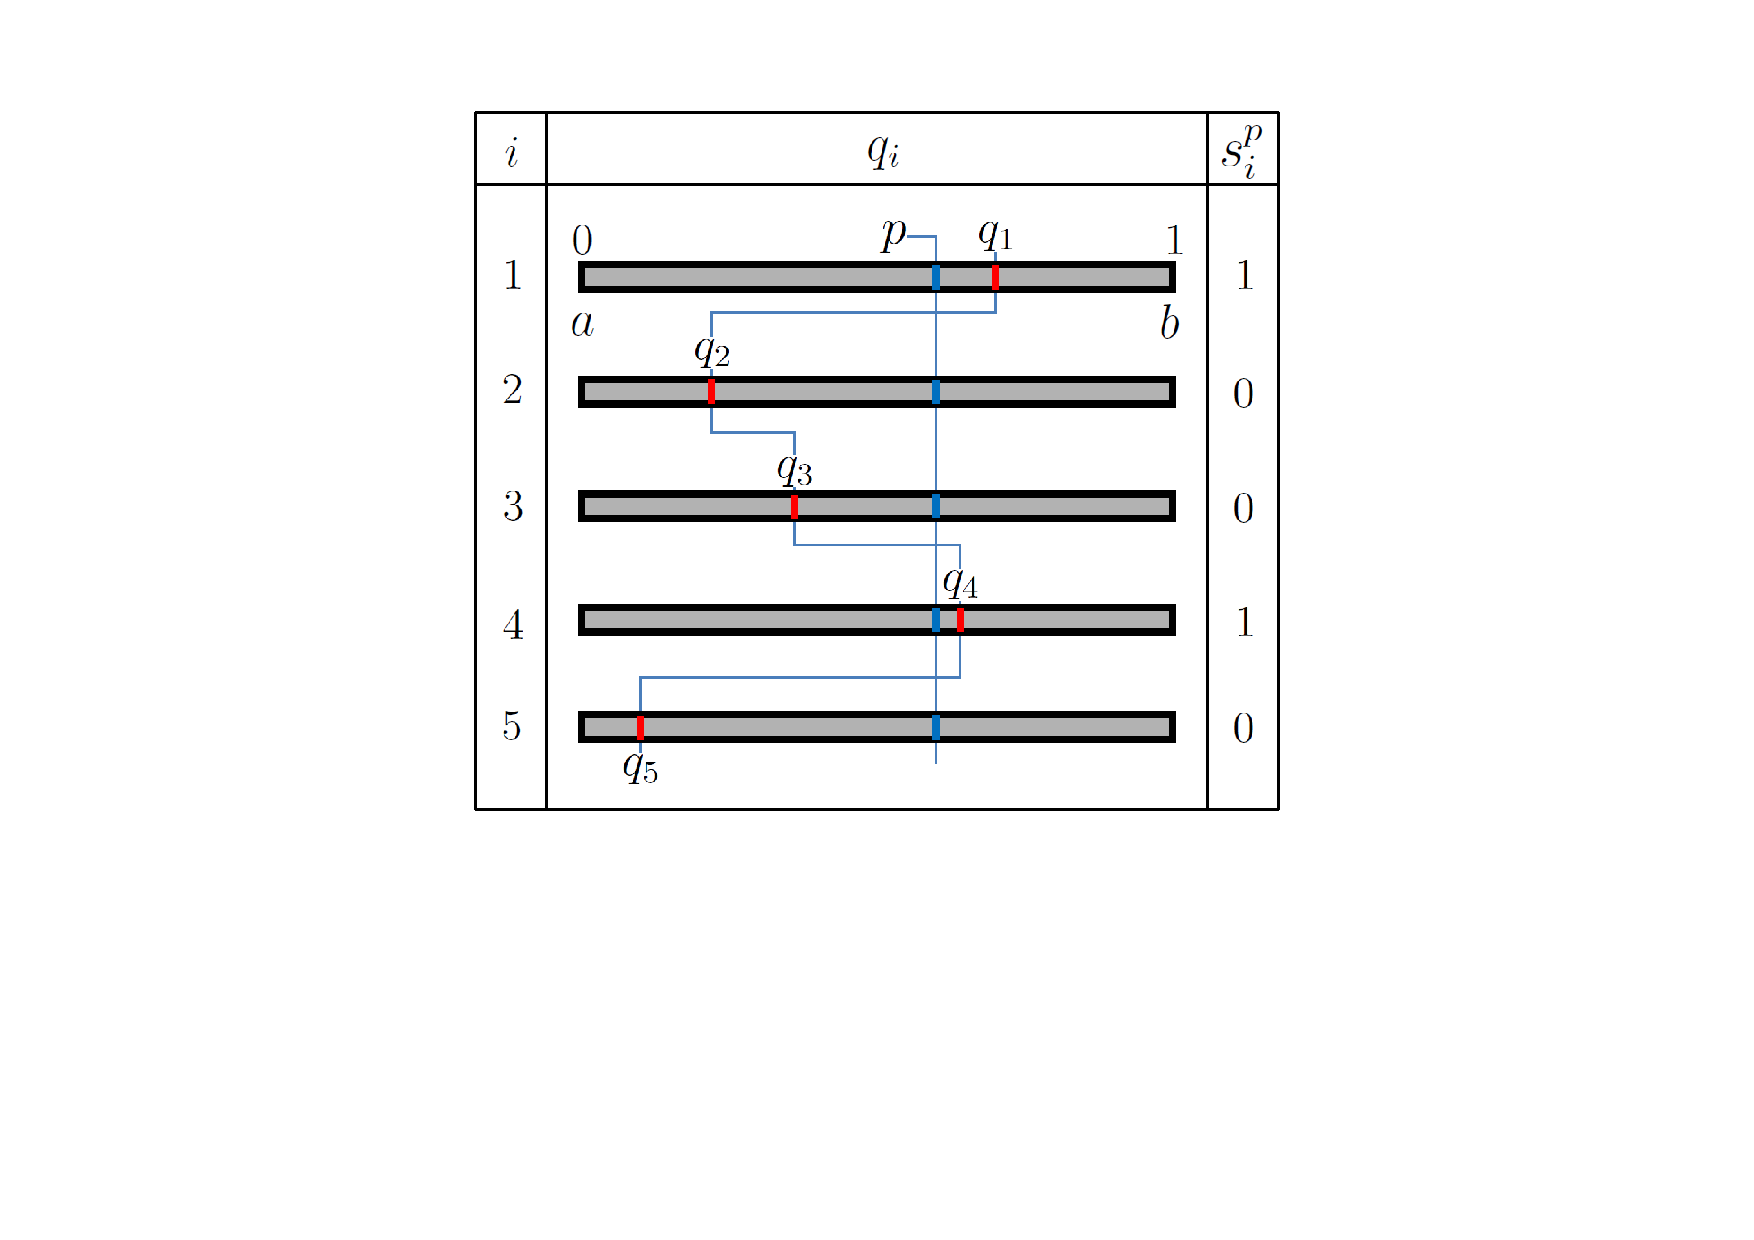
\includegraphics[scale=.5]{sliding-pin-bw}\label{fig:sliding}}
	\caption{Illustration of the operation of two arithmetic-decoding techniques for a string of length $\ell=5$. The leftmost column $i$ of each illustration indicates the decoding step. The corresponding output bit for each step is depicted in  the rightmost column. (a) \emph{Shrinking-interval} decoding \cite{Said04}: The values of $\{[a_i,b_i],p_i\}_{i=1}^{5}$ are updated recursively using Equations \eqref{eq:aibipi} for a given fixed $q$ whilst the output bit $s^q_i$ is obtained with Equation \eqref{eq:spi}; the shaded area within the nested subintervals shrinks away as the decoding progresses. (b) \emph{Sliding-pin} decoding: The support interval and $p$ are now fixed, while $\{q_i\}_{i=1}^{5}$ is subsequently shifted throughout the unit interval using Equation \eqref{eq:qi}, thus resembling the strip of a sliding-rule; the output bit $s^p_i$ in this case is given by Equation \eqref{eq:sqi}.}
	\label{fig:ac}
\end{figure}

\subsection{Truncated-normal random numbers}
Algorithm \ref{alg:TILDA} is designed to work in continuous domains where variables are assumed to be Gaussian-distributed over the real line. In an arithmetic coding scheme, however, the search of a feasible set of values for a pair $(p,q)$ requires the evolutionary algorithm to generate random numbers bounded within the $[0,1]$ interval\footnote{Let us mention that mechanisms for truncated pseudorandom number generation in other support intervals has been also highlighted in previous \EDA~studies (e.g. \cite{Mininno08, Grahl04})}. For this reason we adapted the algorithm to a \emph{truncated} Gaussian model with support on the unit interval only, following \cite[page 39]{Devroye86}: given a random variable $X$ with cumulative probability distribution $\Phi$, the truncated random variable $X^\transpose$ with distribution $\Phi^\transpose$ and support $[a,b]$ is defined as
\begin{equation}\label{eq:phit}
\Phi^\transpose(x) = \left \{ \begin{matrix}
  								 0 & x<a \\
  								 \frac{\Phi(x)-\Phi(a)}{\Phi(b)-\Phi(a)} & a \le x \le b \\
  								 1 & x>b 
 \end{matrix} \right.. 
\end{equation}
We define $\Phi \equiv \gauss{\mu}{\sigma}, a=0, b=1$ and normalise $x'=\tfrac{x-\mu}{\sigma}$, $a'=\tfrac{a-\mu}{\sigma}=\tfrac{-\mu}{\sigma}$ and $b'=\tfrac{b-\mu}{\sigma}=\tfrac{1-\mu}{\sigma}$. Let $u \sim [0,1]$ be a uniformly distributed random number; hence we use the inversion method for random number generation (see e.g.\cite{Devroye86}), that is, assume $u = \Phi^\transpose(x')$ and work out the resulting $x$ bounded to [0,1]. Since $0 \le x' \le 1$ from Equation (\ref{eq:phit}) we get:
$$ \Phi(x') = u(\Phi(b')-\Phi(a'))+\Phi(a'),$$
which in turn implies that,
\begin{equation}
x = \sigma(\Phi^{-1}(u(\Phi(b')-\Phi(a'))+\Phi(a'))+\mu.
\label{eq:trunc}
\end{equation}
Since $\Phi(a')$ and $\Phi(b')$ are constant terms, Equation (\ref{eq:trunc}) can be used to generate a truncated random number by computing a uniform random number and one evaluation of the inverse normal distribution with given parameters $(\mu, \sigma)$.  

\section{Algorithm}
\label{sec:algorithm}
To begin with, let us recall the arithmetic-coded \EDA~proposed in \cite{Suwannik08}. It is a continuous domain population-based \EDA~that takes advantage of the shrinking-interval arithmetic decoding, defined in Equations (\ref{eq:spi}-\ref{eq:aibipi}), in order to search for a solution string $\bs_p^q$ in a high dimensional space of size $\ell$. The compression scheme reduces the memory requirements needed to store and maintain the population of candidates, enabling the algorithm to solve large-scale problems in a standard desktop machine. Here we present an algorithm that further improves memory usage by means of a compact representation. 

The new algorithm is an adaptation of \TILDA~(as described in Section \ref{sec:tilda}). The idea is to search for the best $(p, q) \in \Rdom^2$ that determines the string $\bs_p^q$ whose fitness function is evaluated in $\{0,1\}^\ell$. For this purpose, we let $\bmu, \tilde{\bmu}, \bsigma, \tilde{\bsigma}, \bbeta \in \Rdom^2$ in Algorithm \ref{alg:TILDA} and we chose the sliding-pin scheme of \mbox{Equations (\ref{eq:qi}-\ref{eq:sqi})} to decompress $\bs_p^q$. Likewise, we decided on using the truncated Gaussian random generator of Equation (\ref{eq:trunc}) for sampling. The resulting method (\TILDAC: \emph{arithmetic-coding} \TILDA) is shown in Algorithm \ref{alg:TILDAC}. 

The time complexity of the algorithm is dependent on the convergence speed, the population size $n$, and the cost needed to decompress and evaluate the candidate (usually linear in $\ell$). More specifically, neglecting the cost of random number generation, each inner loop iteration incurs $O(\ell)$ for the two fitness evaluations in line \ref{tildac:fitness} (the fitness evaluations in line \ref{tildac:best} can be spared by caching previous calls). So, assuming $t_c$ iterations are needed to converge, the running time is in $O(n \ell t_c)$. 

\begin{algorithm}
	\caption{\TILDAC} 
	\begin{algorithmic}[1]
	%\REQUIRE{$\bmu, \tilde{\bmu}, \bsigma, \tilde{\bsigma}, \bbeta \in \Rdom^2, \gamma,\epsilon \in \Rdom$, fitness function $f(\cdot)$}
	\REQUIRE{$\ell>0$, fitness function $f(\cdot)$}
	\ENSURE{best candidate $\bbeta$}
		\STATE $\bbeta=\bmu=(0.5,0.5), \bsigma=(10,10), \gamma=0.9, \epsilon=\ell^{-1}$
		\WHILE{\textbf{convergence}} \label{tildac:genloop}
			\STATE $\tilde{\bmu}=\tilde{\bsigma}=(0,0)$
			\FOR{$n$ \textbf{times}} \label{tildac:poploop}
				\STATE $\{(p^{\prime},q^{\prime}), (p^{\prime\prime},q^{\prime\prime})\} \sim  \tgauss{\bmu}{\bsigma}$ {{\scriptsize //sampling (Eq.(\ref{eq:trunc}))}}  %\COMMENT{{\scriptsize /* sampling (Eq.(\ref{eq:trunc})) */}}  
				\STATE $(\hat{p},\hat{q}) = \mathsf{argmax}(f(\bs_{q^{\prime}}^{p^{\prime}}), f(\bs_{q^{\prime\prime}}^{p^{\prime\prime}}))$ {{\scriptsize //decoding (Eq.(\ref{eq:qi}-\ref{eq:sqi})) 
				}} \label{tildac:fitness}
				\STATE $\bbeta = \mathsf{argmax}(f(\bs_{\hat{q}}^{\hat{p}}), f(\bs_{\beta_2}^{\beta_1}))$ {{\scriptsize // update best}} \label{tildac:best}
				\STATE $\tilde{\bmu} = \tilde{\bmu} + \frac{1}{n}(\hat{p},\hat{q})$ \label{tildac:muhat}
				\STATE $\tilde{\bsigma} = \tilde{\bsigma} + \frac{1}{n}(\hat{p}^2,\hat{q}^2)$	 \label{tildac:sigmahat}
			\ENDFOR			
			\STATE $\bmu=\bmu-\gamma(\bmu-\frac{1}{2}(\bbeta+\tilde{\bmu}))$ \label{tildac:mu}
			\STATE $\bsigma=\bsigma-\gamma(\bsigma-(\tilde{\bsigma}-(\tilde{\mu}_0^2, \tilde{\mu}_1^2))+\epsilon$	 \label{tildac:sigma}		
		\ENDWHILE
	\end{algorithmic}  
	\label{alg:TILDAC}
\end{algorithm}

Now we discuss an interesting memory saving mechanism obtainable with this new algorithm. Observe that its memory cost is dominated by the size of the problem $\ell$. This is because the working memory consists of nine bi-dimensional variables in $O(1)$ plus the temporal buffer needed to decompress $\bs_p^q$, which is in $O(\ell)$. However, if we constrain the application domain to additively-separable problems exhibiting modularity of fitness evaluation to the level of single variables, that is, problems where the fitness function aggregates independent contributions in each dimension of the solution, then the memory cost can be $O(1)$. The latter is possible by incrementally evaluating and disposing bits obtained during the stream decompression of $\bs_p^q$. And given that the best solution can be retrieved at any point of the evolutionary loop from the arithmetic code $\bbeta=(\beta_1,\beta_2)$, corresponding to $\bs_{\beta_1}^{\beta_2}$, no string buffering is actually needed. As mentioned earlier, even if bits are not discarded (i.e. buffering them into a string) the fitness evaluation requires $O(\ell)$ time to scan the string, so the memory savings using streaming implies no additional time overload. It is in this sense that the algorithm is well suited for large scale problems, ensuring minimal memory consumption, regardless of the problem and population size. The memory efficiency of \TILDAC~ compares favorably with arithmetic-coded \EDA\cite{Suwannik08}, which requires $O(\ell+n)$ for the evolutionary loop (although it could be lowered to $O(n)$ by using the same streaming technique), and also with \cGA\cite{Harik99}, which requires $O(\ell(\log_2 n+2))$. 

It may be noted in passing that, by using the sliding-pin arithmetic-coding technique and the truncated random number generator, \TILDAC~is able to always decompress feasible solutions notwithstanding the problem size $\ell$. The latter contrasts with the difficulties found for the arithmetic-coded \EDA, where some $(p,q)$ codes where unable to produce the desired string length due to precision issues\cite{Suwannik08}.

\begin{table}
	\centering
	{\footnotesize
	\renewcommand{\arraystretch}{1.6}
		\begin{tabular}{|c|c|}
			\hline
			\textbf{Problem} & \textbf{Fitness function} \\
			\hline \hline 
			\onemax & $f(\bs) = \sum_{i=1}^\ell s_i$ \\
			\hline
			\noisy \onemax & $\hat{f}(\bs) = f(\bs) + \gauss{0}{\sigma^2_N}$ \\
			\hline
			\rroad & $f_c(\bs) = \sum_{i=0}^{(\ell/c)-1} c\left(\prod_{k=ic+1}^{(i+1)c} s_k \right)$ \\
			\hline
			\noisy \rroad & $\hat{f}_c(\bs) = f_c(\bs)+\gauss{0}{\sigma^2_N}$\\
			\hline 
		\end{tabular}
	}
	\caption{Fitness functions used in the empirical study for a candidate $\bs=\{s_1,\ldots,s_{\ell}\}$, $s_i \!\!\in\!\! \{0,1\}$. $\gauss{0}{\sigma^2_N}$ denotes a normally distributed random variable of variance $\sigma^2_N$.} 
	\label{tab:fitfun}		
\end{table}

\begin{table}
	\centering
	{\footnotesize
		\begin{tabular}{|p{6.5cm}|}
		\hline
	\begin{algorithmic}
	\REQUIRE{$(p,q), \ell, noise$}
	\ENSURE{$f$}
		\STATE $f=0$
		\FOR{$\ell$ \textbf{times}} 
			\STATE $bit=q>p$
			\STATE \textbf{if} $bit$ \textbf{then} 
			\STATE $\qquad$ $q=(q-p)/(1-p)$
			\STATE $\qquad$ $f=f+1$
			\STATE \textbf{else} $q=q/p$ 
		\ENDFOR			
		\STATE \textbf{end-repeat}
		\STATE \textbf{if} $noise$ \textbf{then} $f=f+\gauss{0}{\sigma^2_N}$ 
	\end{algorithmic}  
\\
\hspace{2.3cm}(a) \onemax \\ \\
\hline\hline
	\begin{algorithmic}
	\REQUIRE{$(p,q), \ell, c, noise$}
	\ENSURE{$f$}
		\STATE $f=0; k=1; block=\TRUE$
		\FOR{$\ell$ \textbf{times}} 
			\STATE $bit=q>p; \;\;block=block \wedge bit$
			\STATE \textbf{if} $bit$ \textbf{then} $q=(q-p)/(1-p)$
			\STATE \textbf{else} $q=q/p$
			\STATE \textbf{if} $k=c$ \textbf{then}
				\STATE $\qquad$ $k=0$ 
				\STATE $\qquad$ \textbf{if} $block$ \textbf{then} $f=f+c$
				\STATE $\qquad$ \textbf{else} $block=\TRUE$
			\STATE \textbf{end-if}
			\STATE $k=k+1$
		\ENDFOR			
		\STATE \textbf{end-repeat}
		\STATE \textbf{if} $noise$ \textbf{then} $f=f+\gauss{0}{\sigma^2_N}$ 		
	\end{algorithmic}  

\\
\hspace{2.3cm}(b) \rroad \\ \\
\hline

		\end{tabular}
	}
	\caption{Stream algorithms for string decompression and fitness evaluation. (a) \onemax: this algorithm is a variation of the sliding-pin arithmetic decoder of Equations (\ref{eq:qi}-\ref{eq:sqi}), where the fitness $f$ is increased every time the current \emph{bit} is set to \textbf{true}; inputs are: arithmetic code $(p,q)$, problem size $\ell$, and a $noise$ flag to activate the noisy version. (b) \rroad: based on the \onemax~code above, and using $c$ as an additional input defining the order of the schema, this algorithm keeps a $block$ flag that is successively updated with the conjunction of the decoded $bit$ variable; for every succeeding schema, whose extent is controlled with counter $k$, score $c$ is added to $f$ if the schema $block$ flag is set, otherwise this flag is readjusted. } 
	\label{tab:stream}		
\end{table}

\section{Empirical study}
\label{sec:experiments}

We conducted an empirical study of \TILDAC~applied to the \onemax\cite{Pelikan09} and \rroad\cite{Mitchell91} problems (including noisy variations). Fitness functions for a candidate solution ($\bs \in [0,1]^\ell$) to these problems are defined in Table \ref{tab:fitfun}. For the case of \rroad~functions, the parameter $c$ represents a score added to a candidate for each succeeding schema of order $c$ that can be found within its bit string, starting at bit 1 (in contrast to the original definition given in \cite{Mitchell91}, here only a single block scan of $\ell/c$ schemas is carried out to compute fitness; no additional hierarchical scans of higher -doubled- order schemas follow up).

Let us observe that the evaluation of these fitness functions allows additively-separable computations. Hence we implemented stream decompression/fitness-evaluation algorithms (see Table \ref{tab:stream}) in order to take advantage of the memory savings of \TILDAC\footnote{We remark that the algorithm is suitable as well for non-decomposable fitness functions, or problems where no stream decompressing algorithm is available. In the worst of these cases its memory complexity, as mentioned earlier, would be in $O(\ell)$, still a favourable scenario for large-scale applications.}. Instead of $\bs$, these stream algorithms take an arithmetic code $(p,q)$ as their input, which implicitly defines the bit string $\bs_p^q$ of Equation (\ref{eq:spq}), and simultaneously decompress the candidate and compute its fitness value $f$. In this way we were able to run the experiments in a conventional laptop Intel\textregistered~Core\texttrademark~i7 machine with 6GB memory. Algorithm \ref{alg:TILDAC} and test-bed scripts were implemented in both Octave version 3.2.4 with QtOctave version 0.9.1 and Matlab R2011. Fitness routines in Table \ref{tab:stream} were implemented in C with the MEX interface for faster evaluation.

\subsection{Results on noiseless problems}
The first set of experiments were aimed at testing the behaviour of the algorithm on noise-free (regular) problems. We set the number of maximum generations to $1000$ for all experiments, with an early-stopping condition whenever a candidate decoding a number of bits equals to the problem size $\ell$ was found. In order to set the appropriate population size needed to find a solution with respect to $\ell$, we carried out a grid-search \cite{Hsu2003} over $n \in\{2^3,2^4,\ldots,2^{12}\}$; the search was stopped when, for a given $n$, at least 90\% of 100 runs were successful. For the \rroad~case, the schema order $c$ was set to 100 for all experiments. The values of learning rate and premature convergence parameters ($\gamma=0.9$ and $\epsilon=\ell^{-1}$) were chosen from empirical evidence of preliminary experiments. Results of the final experiments are listed in Table \ref{tab:results-noiseless}.

In summary, these results show that the algorithm succeeded in solving both problems from medium- to large-scale lengths ($10^3$ to $10^7$ variables). Interestingly enough, it can be seen that a small population size $n \le 32$ was needed to solve the problems, even for the large dimensionalities. The average generation of solution emergence was much smaller than the maximum setting of 1000. On the other hand, a comparable trend of performance is visible in the \onemax~and \rroad~\mbox{instances}, except that a bigger population size was needed in the smaller problems for the latter. This finding may drop a hint on the potential \mbox{effectiveness} of the algorithm to tackle basic levels of structure in the problem (recall that \rroad fitness function assigns score only to entire schemas of length $c$, that is, contiguous chunks of variables).   

\subsection{Results on noisy problems}
The second set of experiments focused on testing the robustness of the algorithm when exogenous noise was added to the original fitness function. We followed the same settings as before but with 30 runs. Again the population size was obtained by a grid-search. The level of noise was controlled with a exogenous-noise-variance to deterministic-fitness-variance ($\frac{\sigma^2_N}{\sigma^2_f}$) parameter as defined in \cite{Sastry07}. We tested the algorithm using a corruption $\frac{\sigma^2_N}{\sigma^2_f}$ ratio of $10^{-2}$. Results of this set of experiments are listed in Table \ref{tab:results-noisy}.

In these experiments, the results on both problems are dissimilar. For the \mbox{\noisy\onemax}~problem the incidence of noise in medium-size instances causes no difficulty to the algorithm in solving it. In larger instances, however, ($\ell=\{10^5, 10^6\}$) the algorithm struggles and demands higher population sizes of up to $n=2048$ but still obtains success rates inferior to 50\%. In contrast, a small population size $n=32$ seems appropriate to solve all instances of \noisy \rroad~problems. We reason that in this case, the block-structure of the fitness score diminishes the effect external noise may have in misguiding the algorithm during its search. 

\begin{table}
	\centering
	{\footnotesize
	\renewcommand{\arraystretch}{1.2}
		\begin{tabular}{|c||c||c||c|}
		\hline
		Problem & \multirow{2}{*}{Solution} & \multirow{2}{*}{\onemax} & \multirow{2}{*}{\rroad} \\ 
		size & & & \\
		\hline
		\hline
		\multirow{3}{*}{$\ell=10^3$} 
		 & $n$ & 8 & 16  \\
		 & Success rate & 100/100 & 96/100 \\
		 & Age (avg.)  & 29.62 & 58.22 \\
		 %& Bits (avg.) & 1000.00 &  \\
		\hline
		\hline
		\multirow{3}{*}{$\ell=10^4$} 
		 & $n$ & 8 & 16  \\
		 & Success rate & 99/100 &  92/100\\
		 & Age (avg.)  & 77.21 & 42.33 \\
		 %& Bits (avg.) & 9999.99 &  \\
		\hline
		\hline
		\multirow{3}{*}{$\ell=10^5$} 
		 & $n$ & 8 & 16 \\
		 & Success rate & 98/100 & 99/100 \\
		 & Age (avg.)  & 146.58 &  93.24 \\
		 %& Bits (avg.) & 99999.98 &  \\
		\hline
		\hline
		\multirow{3}{*}{$\ell=10^6$} 
		 & $n$ & 16 & 16  \\
		 & Success rate & 94/100 & 94/100 \\
		 & Age (avg.)  & 229.95 &  207.27 \\
		 %& Bits (avg.) & 999999.94 &  \\
		\hline
		\hline
		\multirow{3}{*}{$\ell=10^7$} 
		 & $n$ & 32 & 32  \\
		 & Success rate & 95/100 &  91/100 \\
		 & Age (avg.)  & 214.88 &  235.59 \\
		 %& Bits (avg.) & 9999999.95 &  \\
		\hline
		\end{tabular}
	}
	\caption{Noise-free experiments. For each problem (\onemax, \rroad) and dimension $\ell$, results are reported on $n$ (population size required to solve it), success rate (successful runs over 100 repetitions) and average age of the solution (generation where optimal candidate emerged).} 
	\label{tab:results-noiseless}		
\end{table}

\begin{table}
	\centering
	{\footnotesize
	\renewcommand{\arraystretch}{1.2}
		\begin{tabular}{|c||c||c||c|}
		\hline
		Problem & \multirow{2}{*}{Solution} & \multirow{2}{*}{\onemax} & \multirow{2}{*}{\rroad} \\ 
		size & & & \\
		\hline
		\hline
		\multirow{3}{*}{$\ell=10^3$} 
		 & $n$ & 8 & 32  \\
		 & Success rate & 28/30 & 30/30 \\
		 & Age (avg.)  & 59.93 & 32.20 \\
		\hline
		\hline
		\multirow{3}{*}{$\ell=10^4$} 
		 & $n$ & 64 & 32  \\
		 & Success rate & 30/30 &  30/30\\
		 & Age (avg.)  & 48.17 & 48.47 \\
		\hline
		\hline
		\multirow{3}{*}{$\ell=10^5$} 
		 & $n$ & 2048 & 32 \\
		 & Success rate & 19/30 & 27/30 \\
		 & Age (avg.)  & 134.37 &  133.90 \\
		\hline
		\hline
		\multirow{3}{*}{$\ell=10^6$} 
		 & $n$ & 2048 & 32  \\
		 & Success rate & 12/30 & 28/30 \\
		 & Age (avg.)  & 168.87 &  153.80 \\
		\hline
		\end{tabular}
	}
	\caption{Noisy experiments. An exogenous noise rate of $\frac{\sigma^2_N}{\sigma^2_f}=0.01$ was used in both test problems. For each each problem (\onemax, \rroad) and dimension $\ell$, results are reported on $n$ (population size required to solve it), success rate (successful runs over 30 repetitions) and average age of the solution (generation where optimal candidate emerged).} 
	\label{tab:results-noisy}		
\end{table}

\section{Conclusions}
\label{sec:conclusion}
We introduced a new compact \EDA~algorithm that is able to solve to optimality additively-separable bit-string problems of up to $10^7$ dimensions with minimum memory requirements, both at individual or block contribution of variables to the fitness score. In the presence of noise, the algorithm is suitable to solve medium to large-size instances of \noisy \rroad~problems but struggles with large scale \noisy\onemax~problems.  On this topic we are considering exploring different ideas for noise tolerance such as the effect of using a combination of best candidates obtained from independent shorter, quicker runs, and also analysing in depth the role of elitism in such scenario.

In addition we are planning to study the role of the learning rate and premature convergence parameters within more elaborated mechanisms as those proposed in existing \EDA~literature. Moreover, it would be interesting to study the behaviour of the algorithm in different kinds of fitness landscapes, for example, uneven (not all-ones) optimal solutions and also, deceptive functions. Yet another  exciting avenue of future research is extending the memory and time efficiency ideas here presented to models of higher-order variable interaction. 

As a concluding remark we anticipate that a parallel implementation of the algorithm would improve running times, although at present, an average run to solve a one-million bit problem in a regular laptop with a population size of 2048 is 1 hour. Our current work aims to validate and extend these findings to very-high dimensional problems of up to one-billion variables.

\section{Acknowledgments}
We would like to thank the anonymous reviewers for their insightful comments and suggestions.

\bibliographystyle{abbrv}
\bibliography{biblio}  
\vfill
\end{document}
